% Ch1Introduction.tex

\chapter[Introduction]{Introduction}
\label{cha:cha1Introduction}

%=============
\section{Motivation and background}
During the past decades, rapid decreases in frog populations have been spotted from locations over the world, which are regarded as one of the most critical threats to the global biodiversity. Many environment problems are regarded as the reasons for these declines: disease, habitat destruction and modification, exploitation, pollution, pesticide use, introduced species, and ultraviolet-B radiation (UV-B). 
On one hand frog populations are rapidly worldwide declining, and on the other frogs are greatly important to the global ecosystem. 
\begin{enumerate}
\item[(1)] Frogs are integral part of the food web
\item[(2)] Frogs are often used as the environment indicators 
\item[(3)] Frogs are important in medical research that benefits humans 
\end{enumerate}

For those aforementioned reasons, increasing frog populations and optimising the protection policy necessitates monitoring of frogs. Frogs are often much easier to be heard than to be seen (Figure.~\ref{fig:Ch1_frogs}). Also frog vocalizations are often employed for most communication, which offer a possible way to study and evaluate frog populations by detecting species-specific calls \citep{dorcas2009auditory}. Therefore, frogs are often monitored via their vocalisations. Traditional manual monitoring methods require ecologists and volunteers to spend extensive time in the field for collecting acoustic data. Although traditional methods can provide an accurate measure of daytime species and richness, it has a limitation in monitoring frog populations over large spatial and temporal scales.
To address this limitation, recent advances in acoustic sensors provide a way to automatically survey vocal animals (such as frogs). Deploying acoustic sensors in the field, frog vocalisations can then be automatically collected. Compared with the manual point-counting method, sensors can greatly extend the survey into larger spatial and temporal scales, and generate large volumes of acoustic data that needs to be analysed. Consequently, enabling automatic species identification in acoustic data has become important. However, because the recordings are automatically collected from the field, the audio data tends to be very noisy. Very often the desired signal (frog call) is weak, and there are multiple overlapping signals over the frog call. Furthermore, different frog species tend to call together to make chorus. All those characteristics pose a big challenge to automatic frog vocalisations survey.

\begin{figure}[htb!]
\centering
      \begin{subfigure}[b]{0.5\textwidth}
           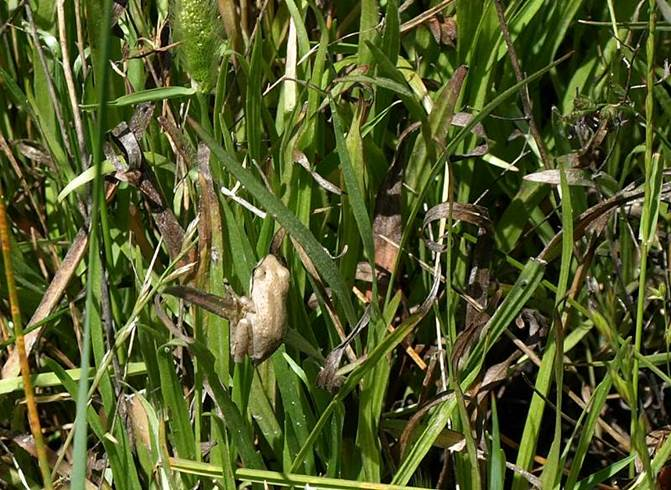
\includegraphics[width=1\textwidth,height=0.75\textwidth]{image/Ch1/unseen_frog_1.jpg}
    \end{subfigure}%
	~~
	      \begin{subfigure}[b]{0.5\textwidth}
           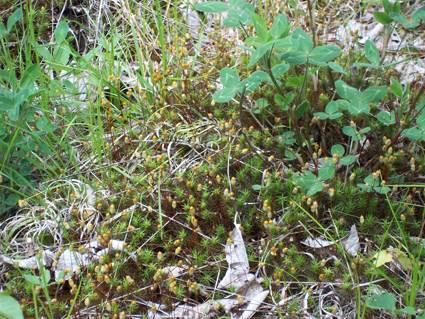
\includegraphics[width=1\textwidth,height=0.75\textwidth]{image/Ch1/unseen_frog_2.jpg}
    \end{subfigure}%
\caption[Photos of frogs]{Photos of frogs to indicate that frogs are difficult to be seen in the field}
\label{fig:Ch1_frogs}       % Give a unique label
\end{figure}



%===============
\section{Basic concepts} 

\subsection{Environment audio data}
The audio data used in this study is mainly derived from two sources: David Stewart's CD \citep{CD} and recordings collected by James Cook University (JCU) \footnote{All the recordings can be obtained from our group website: https://www.ecosounds.org/}. David Stewart's CD is used for the preliminary testing, which is used for the experiment in Chapters \ref{cha:cha4EnhancedFeature} and \ref{cha:cha5Wavelet}. Recordings collected by JCU are used for Chapters \ref{cha:cha6MIML} and \ref{cha:cha7ML}. Firstly, since almost all prior work studied frog recordings with an assumption that only one frog species exists in each individual frog recording, the experiments in Chapter \ref{cha:cha4EnhancedFeature} and \ref{cha:cha5Wavelet} aim to develop a state-of-the-art frog call classification system under this assumption. Secondly, Chapters \ref{cha:cha6MIML} and \ref{cha:cha7ML} focus on the  
study of recordings including multiple overlapping frog vocalisations, which is the real situation for most environment audio data. 


Compared with audio data collected in the laboratories and quiet places (such as David Stewart’s CD), environmental audio data are normally collected under unconstrained noisy conditions (such as JCU recordings). Consequently, the noise and variability issues need to be considered when dealing with environmental audio data. For the background noise, there are a wide variety of non-biological noises and a variety of animal sounds in the environmental recordings. These non-biological noises often come from different sources: rain, wind, human activities (e.g. traffic noise). Besides non-biological noises, many competitive animal sounds (e.g. birds when we are interested in frogs) are also recorded in the environmental audio recordings. In the case of variability, it is produced in many aspects: call structure between species, population of one specific species, time and season changes. All those noises and variabilities make it a challenge to develop a robust frog call classification system.




\subsection{Audio data analysis}
Audio data is usually considered as a mono-dimensional signal. To ease the tasks of understanding, comparison, modification, and resynthesise of signals \citep{rocchesso2003introduction}, audio data analysis is often developed to find the major features representing the time-varying audio data. Many application areas of audio data analysis have been identified: speech processing, mechanical signal processing, bioacoustics analysis, etc. Two most important audio data analysis techniques are Short-time Fourier Transform (STFT) and Linear Predictive Coding (LPC). STFT is a Fourier-related transform, which determines the sinusoidal frequency and phase content of local sections of a signal as it changes over the time \citep{allen1997short}. LPC is mostly used to represent the spectral envelope of an audio data based on the information of a linear predictive model \citep{deng2003speech}. An example of a spectrogram of frog calls derived from a field recording is shown in Figure.~\ref{fig:Ch1_spectrogram}.

\begin{figure}[htb!]
\centering
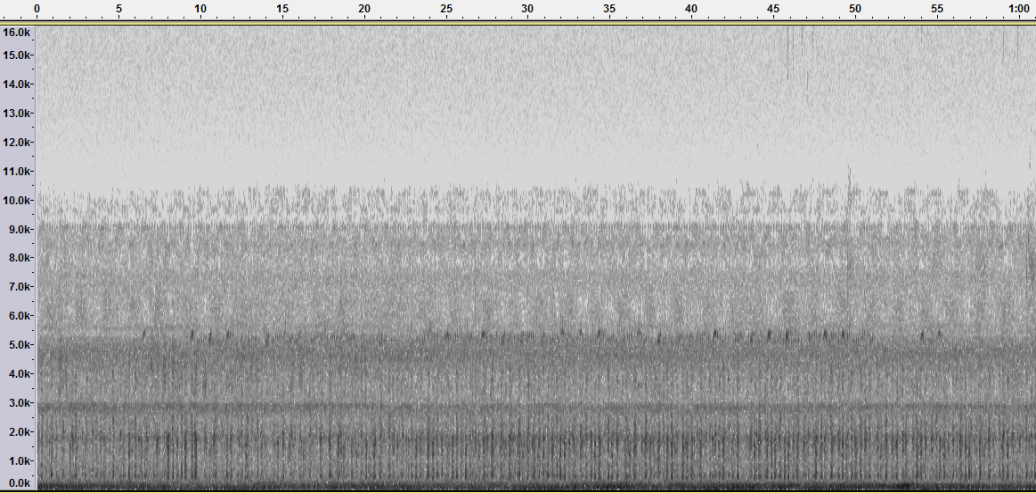
\includegraphics[width=\textwidth]{image/Ch1/spectrogram_example.png}
\caption[An example of spectrogram of environmental recording]{An example of spectrogram of environmental recording. The x-axis is time (seconds); the y-axis is frequency (kHz). The spectrogram is generated from a one-minute recording collected in Townsville, Queensland on around 11.50 pm February 03 2013; the frog species in this recording is \textit{Litoria caerulea}}
\label{fig:Ch1_spectrogram}
\end{figure}





%===================
\subsection{Frog call structure}
Spectrogram (also called sonogram) is a widely used tool for most bioacoustics analysis for its flexible implementation and good applicability. Compared with the hierarchical structure of bird calls, frog calls have a relatively simple call structure \citep{somervuo2006parametric}. The frog vocalisation structure mainly has two ingredients: call and syllable. A frog call is normally made up of several frog syllables (Figure.~\ref{fig:Ch1_spec_mark}).

\begin{figure}[htb!]
\centering
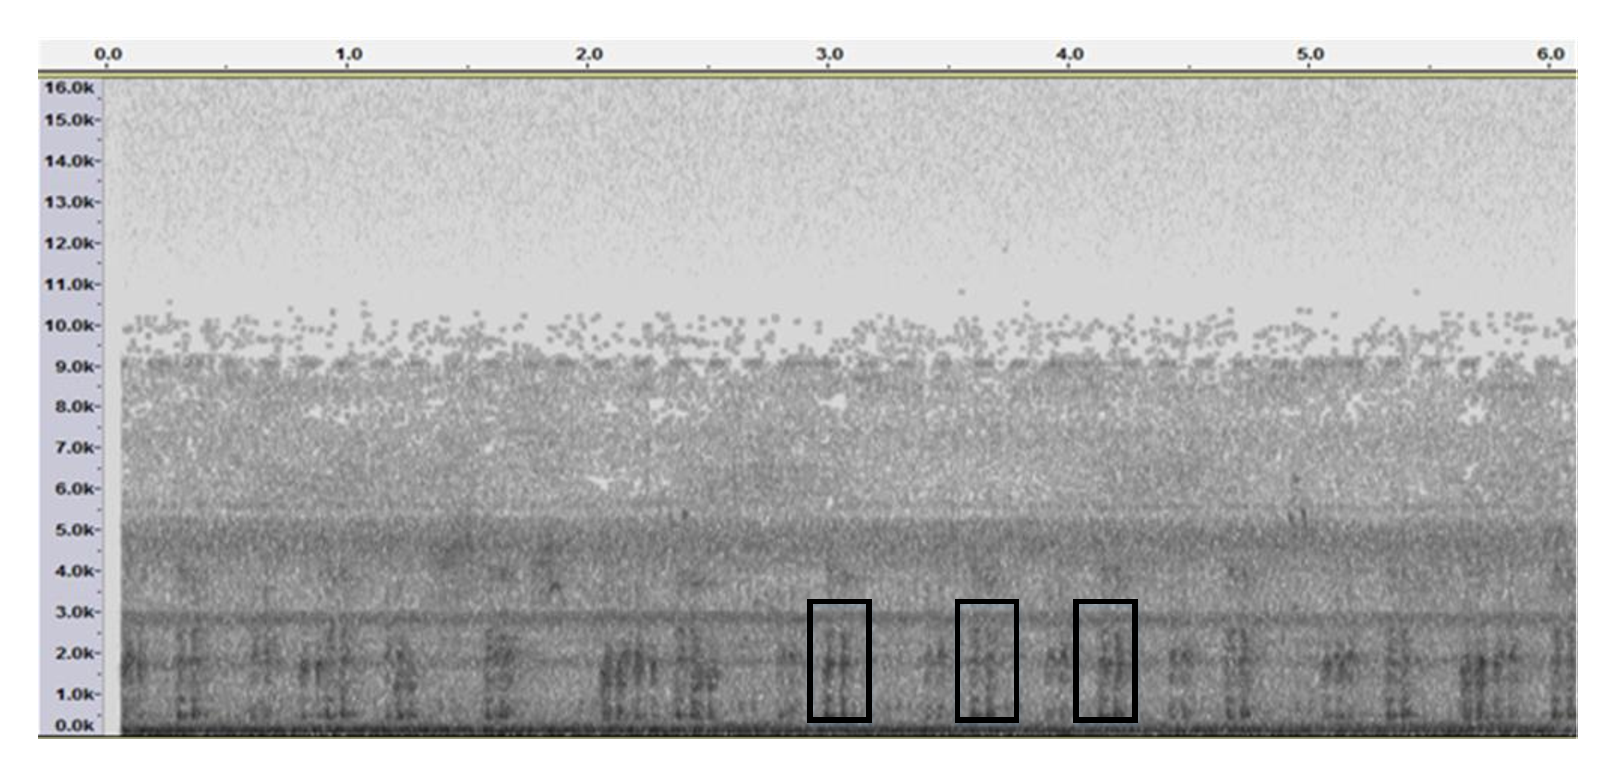
\includegraphics[width=\textwidth]{image/Ch1/spectrogram_mark.pdf}
\caption[Spectrogram of \textit{Litoria caerulea}]{Spectrogram of \textit{Litoria caerulea}, three syllable of \textit{Litoria caerulea} are annotated with one black rectangle, respectively.}
\label{fig:Ch1_spec_mark}
\end{figure}




One syllable is basically a sound that a frog produces with a single blow of air from the lungs \citep{huang2009frog}. For frog call classification, an elementary unit is one syllable. To get an intuitive sense of frog call structure, examples of different frog species in both waveform , spectrogram, and signal-to-noise ratio (SNR) are shown in Table~\ref{tab:wav_spec_cd} and Table~\ref{tab:JCU_para}. For the waveform, x-axis and y-axis represent time and amplitude scales, respectively. The x-axis and y-axis of the spectrogram represent the time and frequency scales, respectively. The grey scale represents the acoustic intensity. Six frog species, which are widely distributed in Queensland, Australia, are selected from David Stewart's CD to generate waveform and spectrogram \citep{CD}. For JCU recordings, eight frog species are selected. The SNR is calculated as follows:

\begin{equation}
SNR=10*log_{10}(\frac{\sum_{i=m}^{m+L}S_{i}^2}{\sum_{j=n}^{n+L}N_{j}^2})
\end{equation}
where $L$ is the length of the signal and noise used for calculating SNR, and set at 6000 samples here, $n$ and $m$ are manual selected start location in the waveform for noise and signal, respectively. 



\begin{table}[htb!]
\centering
\caption[Waveform, spectrogram, and SNR of CD]{Waveform, spectrogram, and SNR of selected six frog species from David Stewart's CD}
\label{tab:wav_spec_cd}
\begin{tabular}{llll}
\hline\hline
\backslashbox{Frog \\ species}{}        & Waveform & Spectrogram & SNR (dB)   \\ \hline
Bufo marinus        &   
\begin{minipage}{.3\textwidth} 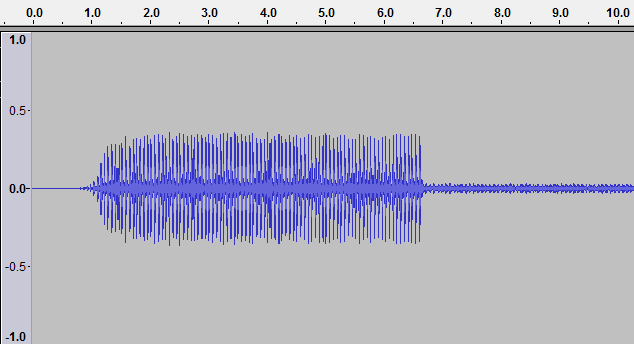
\includegraphics[width=45mm, height=30mm]{image/Ch1/toad_wave.png}  \end{minipage}    &   \begin{minipage}{.3\textwidth} 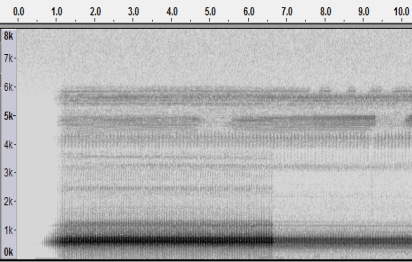
\includegraphics[width=45mm, height=30mm]{image/Ch1/toad_spec.png}  \end{minipage}          & 19.35 \\ \hline
Litoria caerulea    &  \begin{minipage}{.3\textwidth} 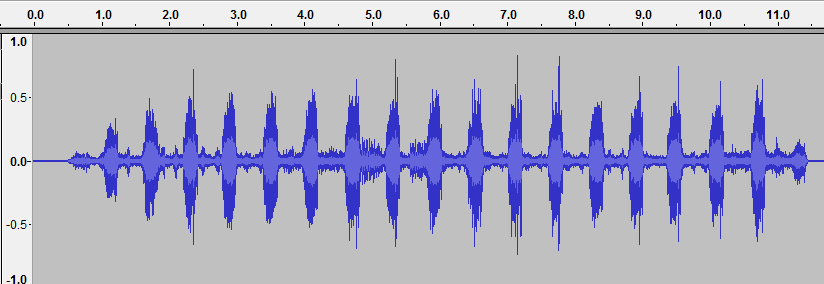
\includegraphics[width=45mm, height=30mm]{image/Ch1/caerulea_wav.png}  \end{minipage}      &     \begin{minipage}{.3\textwidth} 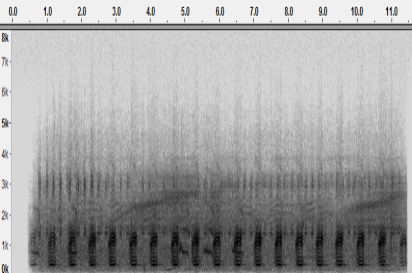
\includegraphics[width=45mm, height=30mm]{image/Ch1/caerulea_spec.png}   \end{minipage}     & 15.78 \\ \hline
Litoria fallax      &      \begin{minipage}{.3\textwidth} 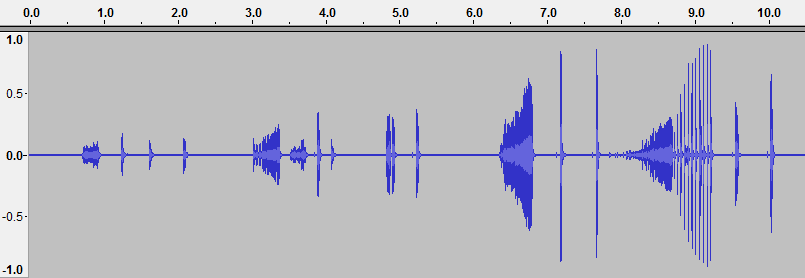
\includegraphics[width=45mm, height=30mm]{image/Ch1/fallax_wav.png} \end{minipage}   &   \begin{minipage}{.3\textwidth} 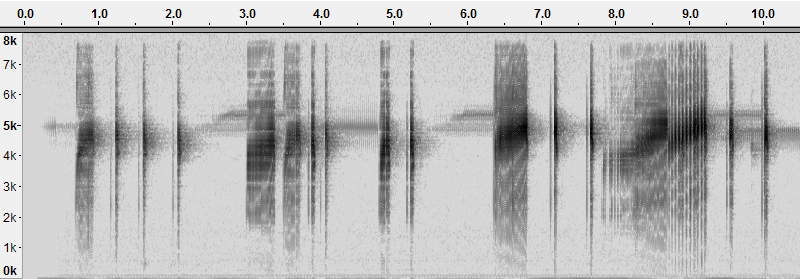
\includegraphics[width=45mm, height=30mm]{image/Ch1/fallax_spec.png}   \end{minipage}       & 43.7  \\ \hline
Litoria gracillenta &     \begin{minipage}{.3\textwidth} 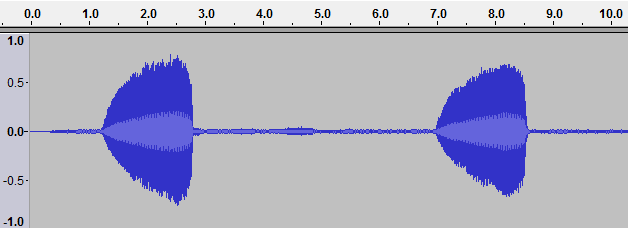
\includegraphics[width=45mm, height=30mm]{image/Ch1/graci_wav.png}  \end{minipage}   &    \begin{minipage}{.3\textwidth} 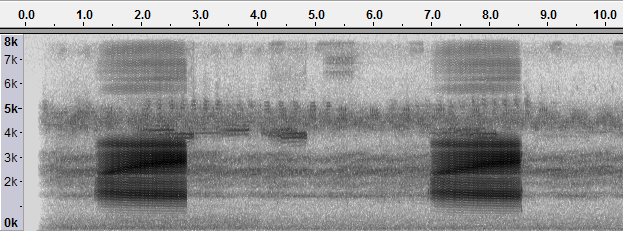
\includegraphics[width=45mm, height=30mm]{image/Ch1/graci_spec.png}     \end{minipage}    & 25.8  \\ \hline
Litoria latopalmata &      \begin{minipage}{.3\textwidth} 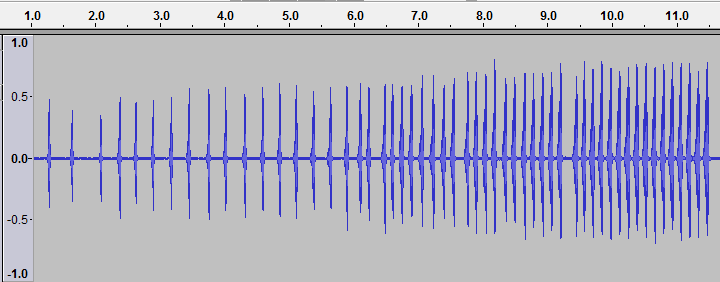
\includegraphics[width=45mm, height=30mm]{image/Ch1/latop_wav.png}  \end{minipage}  &    \begin{minipage}{.3\textwidth} 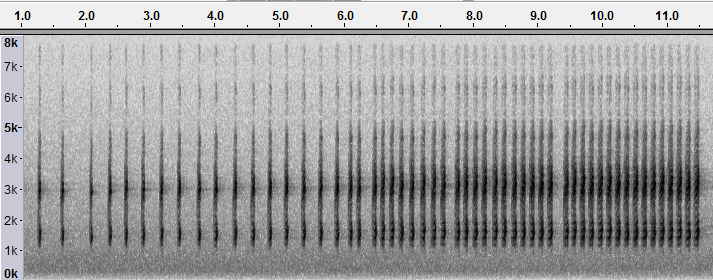
\includegraphics[width=45mm, height=30mm]{image/Ch1/latop_spec.png}    \end{minipage}     & 35.85 \\ \hline
Litoria rubella     &   \begin{minipage}{.3\textwidth} 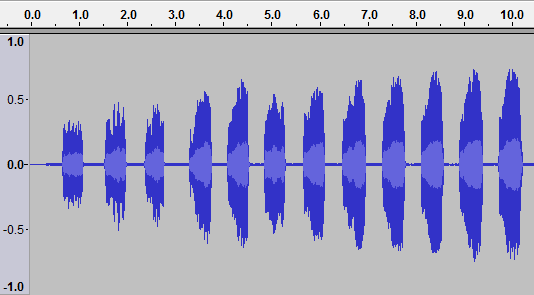
\includegraphics[width=45mm, height=30mm]{image/Ch1/rubella_wav.png}   \end{minipage}    &       \begin{minipage}{.3\textwidth} 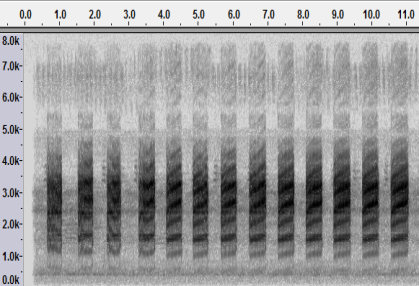
\includegraphics[width=45mm, height=30mm]{image/Ch1/rubella_spec.png}   \end{minipage}   & 36.2  \\ \hline\hline
\end{tabular}
\end{table}



\begin{table}[htb!]
\centering
\caption[Waveform, spectrogram, and SNR of JCU recordings]{Waveform, spectrogram, and SNR of eight frog species (recordings from JCU)}
\label{tab:JCU_para}
\resizebox{\textwidth}{!}{
\begin{tabular}{llll}
\hline\hline
                            & Waveform & Spectrogram & SNR (dB) \\ \hline
Bufo marinus                &   \begin{minipage}{.3\textwidth} 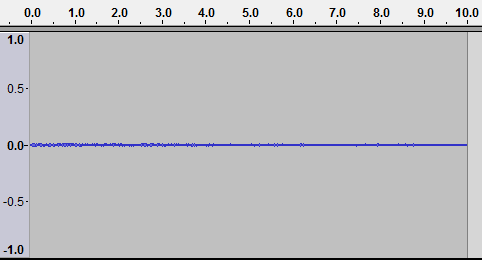
\includegraphics[width=45mm, height=30mm]{image/Ch1/toad_jcu_wav.png}  \end{minipage}       &      \begin{minipage}{.3\textwidth} 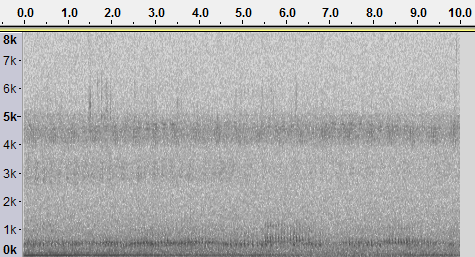
\includegraphics[width=45mm, height=30mm]{image/Ch1/toad_jcu_spec.png}  \end{minipage}       & 1.86     \\ \hline
Cyclorana novaehollandiae   &  \begin{minipage}{.3\textwidth} 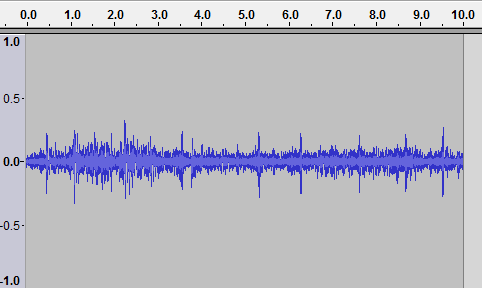
\includegraphics[width=45mm, height=30mm]{image/Ch1/cyc_jcu_wav.png}  \end{minipage}        & \begin{minipage}{.3\textwidth} 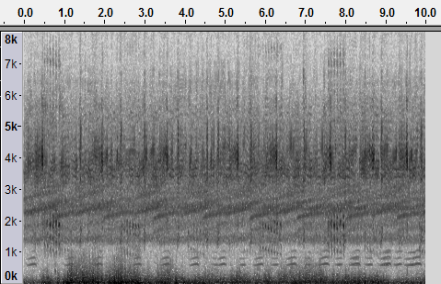
\includegraphics[width=45mm, height=30mm]{image/Ch1/cyc_jcu_spec.png}  \end{minipage}            & -0.13    \\ \hline
Limnodynastes terraereginae &  \begin{minipage}{.3\textwidth} 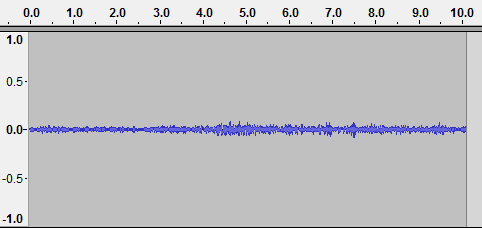
\includegraphics[width=45mm, height=30mm]{image/Ch1/ter_jcu_wav.png}  \end{minipage}        &   \begin{minipage}{.3\textwidth} 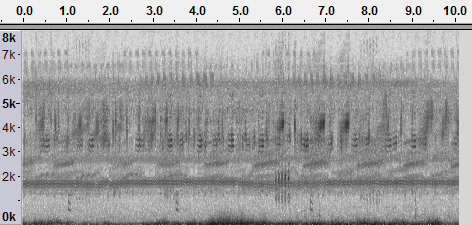
\includegraphics[width=45mm, height=30mm]{image/Ch1/ter_jcu_spec.png}  \end{minipage}          & -2.88    \\ \hline
Litoria fallax              &   \begin{minipage}{.3\textwidth} 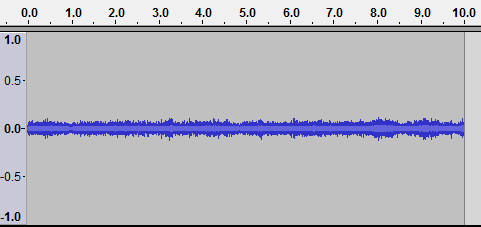
\includegraphics[width=45mm, height=30mm]{image/Ch1/fallax_jcu_wav.png}  \end{minipage}       &    \begin{minipage}{.3\textwidth} 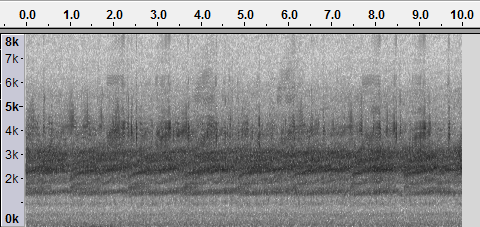
\includegraphics[width=45mm, height=30mm]{image/Ch1/fallax_jcu_spec.png}  \end{minipage}         & 1.52     \\ \hline
Litoria nasuta              &   \begin{minipage}{.3\textwidth} 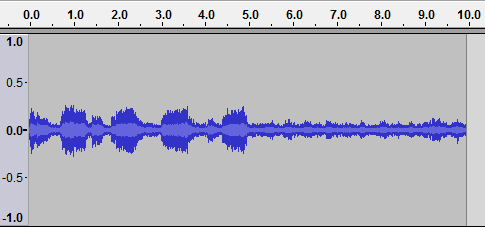
\includegraphics[width=45mm, height=30mm]{image/Ch1/nasuta_jcu_wav.png}  \end{minipage}       &  \begin{minipage}{.3\textwidth} 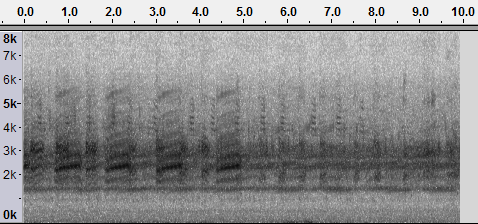
\includegraphics[width=45mm, height=30mm]{image/Ch1/nasuta_jcu_spec.png}  \end{minipage}           & 2.14     \\ \hline
Litoria rothii              &   \begin{minipage}{.3\textwidth} 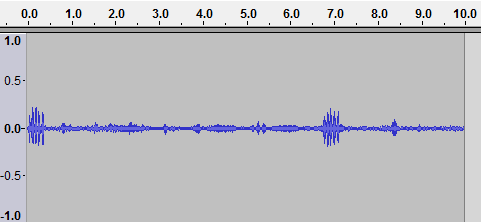
\includegraphics[width=45mm, height=30mm]{image/Ch1/rothii_jcu_wav.png}  \end{minipage}       &    \begin{minipage}{.3\textwidth} 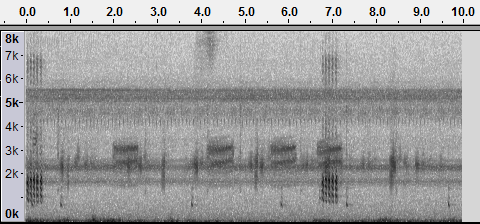
\includegraphics[width=45mm, height=30mm]{image/Ch1/rothii_jcu_spec.png}  \end{minipage}         & 10.24    \\ \hline
Litoria rubella             &    \begin{minipage}{.3\textwidth} 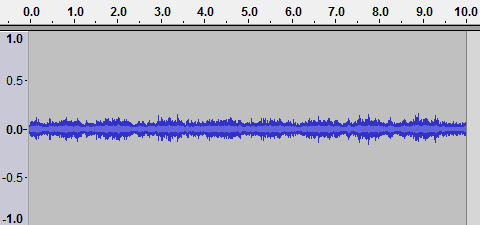
\includegraphics[width=45mm, height=30mm]{image/Ch1/rubella_jcu_wav.png}  \end{minipage}      &   \begin{minipage}{.3\textwidth} 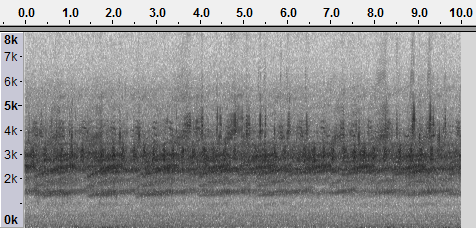
\includegraphics[width=45mm, height=30mm]{image/Ch1/rubella_jcu_spec.png}  \end{minipage}          & 1.08     \\ \hline
Uperolela mimula            &   \begin{minipage}{.3\textwidth} 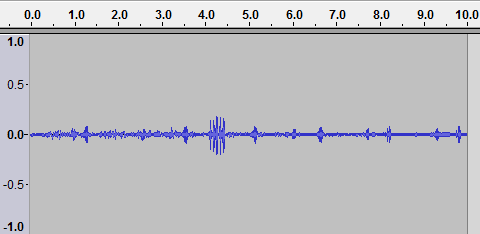
\includegraphics[width=45mm, height=30mm]{image/Ch1/mimula_jcu_wav.png}  \end{minipage}       &  \begin{minipage}{.3\textwidth} 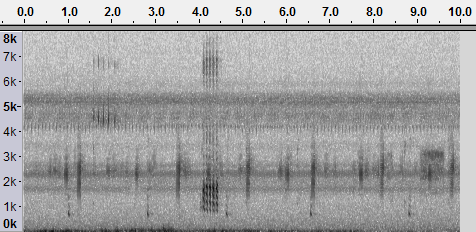
\includegraphics[width=45mm, height=30mm]{image/Ch1/mimula_jcu_spec.png}  \end{minipage}           & 10.28    \\ \hline\hline
\end{tabular}
}
\end{table}


\noindent The parameters of those frog species are shown in Table \ref{tab:cd_parameter}.


\begin{table}[htb!]
\centering
\caption[Averaged parameters of CD]{Averaged parameters of ten syllables of six frog species (David Stewart's CD)}
\label{tab:cd_parameter}
\resizebox{\textwidth}{!}{
\begin{tabular}{llll}\hline\hline
 \backslashbox{Frog \\ species}{Parameters}     & \begin{tabular}[c]{@{}l@{}}Syllable duration \\ (milliseconds)\end{tabular} & Dominant frequency (Hz) & \begin{tabular}[c]{@{}l@{}} Oscillation rate \\ (cycle/second) \end{tabular} \\\hline
Bufo marinus        &    NA   &   600 $\pm$ 30      &                                15 $\pm$ 5 \\
Litoria caerulea    &     500 $\pm$ 30                             &                        500 $\pm$ 75 &    50 $\pm$ 10                             \\
Litoria fallax      &        430 $\pm$ 25                          &                        4700 $\pm$ 450 &                70 $\pm$ 10                 \\
Litoria gracillenta &     430 $\pm$ 25                             &                        4700 $\pm$ 450 &                  70 $\pm$ 10               \\
Litoria latopalmata &       30 $\pm$ 5                           &                        1400 $\pm$ 120 &       5 $\pm$ 2                          \\
Litoria rubella     &   160 $\pm$ 15                               &                        4100 $\pm$ 380 &                            70 $\pm$ 10    \\\hline\hline
\end{tabular}
}
\end{table}




Since the signal power and background noise in this study vary from recordings to recordings and calls to calls within the recording, Table~\ref{tab:CI_CD} and Table~\ref{tab:CI_JCU} calculate the confidence intervals of high and low SNR recordings for the power of signal and noise. The calculation of confidence interval is defined as follows:

\begin{equation}
CI=\mu \pm Z*\frac{\sigma}{\sqrt{L}}
\end{equation}
where $\mu$ and $\sigma$ are the mean and standard deviation, respectively, $Z$ is the upper $\frac{(1-C)}{2}$ critical value for the standard normal distribution, $C$ is the confidence level, and set at 0.95.




\begin{table}[htb!]
\centering
\caption[Confidence interval for CD]{Confidence interval of signal and noise (David Stewart's CD)}
\label{tab:CI_CD}
\begin{tabular}{lll}
\hline\hline
    \backslashbox{Frog \\ species}{Parameters}                      & Confidence intervals of signal & Confidence intervals of noise \\ \hline
Bufo marinus        &  -9.27*$10^{-6}$ $\pm$ 2.10*$10^{-3}$ &  -2.67*$10^{-5}$ $\pm$ 2.26*$10^{-4}$                             \\ 
Litoria caerulea    &      -6.73*$10^{-5}$ $\pm$ 2.40*$10^{-3}$     &                              -6.89*$10^{-5}$ $\pm$ 3.90*$10^{-4}$ \\ 
Litoria fallax      &   -5.85*$10^{-6}$ $\pm$ 1.50*$10^{-3}$                             &                              -2.73*$10^{-5}$ $\pm$ 9.62*$10^{-6}$ \\ 
Litoria gracillenta &     -7.12*$10^{-5}$ $\pm$ 2.00*$10^{-3}$                           &                              -7.70* $10^{-5}$ $\pm$ 1.00*$10^{-4}$ \\ 
Litoria latopalmata &   -6.58*$10^{-5}$ $\pm$ 2.70*$10^{-3}$                            &                              -1.02*$10^{-4}$ $\pm$ 4.36*$10^{-5}$ \\ 
Litoria rubella     &   -3.13*$10^{-5}$ $\pm$ 3.00*$10^{-3}$                           &                              -9.87*$10^{-5}$ $\pm$ 4.70*$10^{-5}$ \\ \hline\hline
\end{tabular}
\end{table}




\begin{table}[htb!]
\centering
\caption[Confidence interval for JCU recordings]{Confidence interval of signal and noise for JCU recordings}
\label{tab:CI_JCU}
\begin{tabular}{lll}
\hline\hline
   \backslashbox{Frog \\ species}{Parameters}                          & Confidence intervals of signal & Confidence intervals of noise \\ \hline
Bufo marinus                &   -1.36*$10^{-5}$ $\pm$ 6.00*$10^{-5}$                             &                              -3.22*$10^{-5}$ $\pm$ 4.80*$10^{-5}$ \\ \hline
Cyclorana novaehollandiae   &    1.30*$10^{-3}$ $\pm$ 8.70*$10^{-4}$                            &                              1.30*$10^{-3}$ $\pm$ 8.90*$10^{-4}$ \\ \hline
Limnodynastes terraereginae &       6.43*$10^{-5}$ $\pm$  1.30*$10^{-4}$                         &                              1.86*$10^{-4}$ $\pm$ 1.89*$10^{-4}$ \\ \hline
Litoria fallax              &  2.31*$10^{-5}$ $\pm$ 5.00*$10^{-4}$                              &                              5.75*$10^{-6}$ $\pm$ 4.22*$10^{-4}$ \\ \hline
Litoria nasuta              &                  -1.55*$10^{-4}$ $\pm$ 4.90* $10^{-4}$              &                              6.25* $10^{-6}$ $\pm$ 3.85*$10^{-4}$ \\ \hline
Litoria rothii              &              -3.32*$10^{-4}$ $\pm$ 9.2*$10^{-4}$                  &                              1.61* $10^{-4}$ $\pm$ 2.84*$10^{-4}$ \\ \hline
Litoria rubella             &      -8.15*$10^{-5}$ $\pm$ 5.52*$10^{-4}$                          &                              -2.69* $10^{-5}$ $\pm$ 4.87*$10^{-4}$ \\ \hline
Uperolela mimula            &             -1.20*$10^{-3}$  $\pm$ 1.10*$10^{-3}$                   &                              -9.36*$10^{-4}$ $\pm$ 3.35*$10^{-4}$ \\ \hline\hline
\end{tabular}
\end{table}




\subsection{Acoustic event and background noise}


An acoustic event is a localised region of high intensity in a spectrogram. As we can see from Figure.~\ref{fig:label}, there are lots of acoustic events in one-minute recording. This study focuses on the frog vocalisations, and frog calls are recorded as signals. Consequently, all the other events are called background noise, whose definition is ambiguous. In this study, both high and low SNR recordings are investigated to build a robust frog call classification system. Most previous studies present the frog call classification system using the high SNR recordings. The high SNR recordings often assume that there is only one frog species in each individual recording with few background noises ($SNR \geq 15 dB$). In contrast, most low SNR recordings consist of more than one frog species in an individual recording with lots of background noises ($SNR \leq 15 dB$). For the low SNR recordings, Table~\ref{tab:psd} show the power spectral density of signal and noise. It can be seen that the noises in low SNR recordings are often generated by several sources and broadband, which cover different frequency bands and lead to the frequency overlapping between the signal and noise. Therefore, it is challenging to analyse the recordings containing background noise and simultaneous vocalising events.




\begin{table}[htb!]
\centering
\caption[PSD of JCU recordings]{Power spectral density (PSD) estimate of signal and noise (JCU recordings); for some frog species, the PSD difference between the signal and background noise is marked with the red rectangle, which indicates the frequency location of specific frog species; for others, the PSD of signal and noise is very similar, which means that some sources have similar frequency information with frog species}
\label{tab:psd}
\resizebox{\textwidth}{!}{
\begin{tabular}{lll}
\hline\hline
  \backslashbox{Frog \\ species}{Parameters}                           & Welch PSD (Signal) & Welch PSD estimate (Noise) \\ \hline
Bufo marinus                &  \begin{minipage}{.3\textwidth} 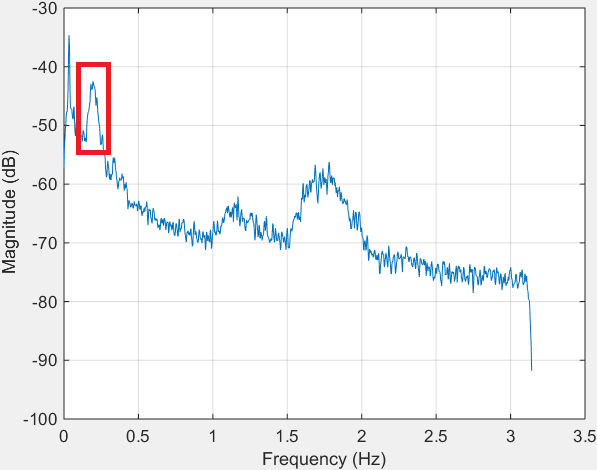
\includegraphics[width=45mm, height=35mm]{image/Ch1/1_signal.png}  \end{minipage}       &      \begin{minipage}{.3\textwidth} 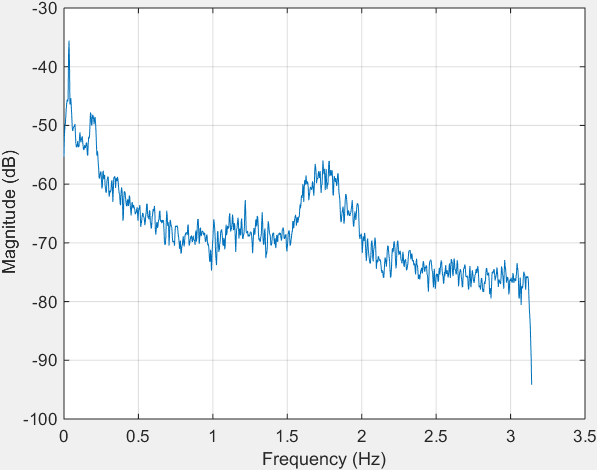
\includegraphics[width=45mm, height=35mm]{image/Ch1/1_noise.png}  \end{minipage}          \\ \hline
\begin{tabular}[c]{@{}l@{}} Cyclorana \\ novaehollandiae  \end{tabular}    & \begin{minipage}{.3\textwidth} 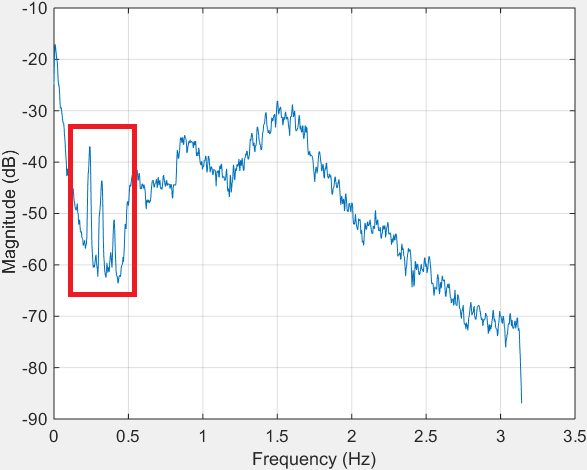
\includegraphics[width=45mm, height=35mm]{image/Ch1/2_signal.png}  \end{minipage}                              &                                              \begin{minipage}{.3\textwidth} 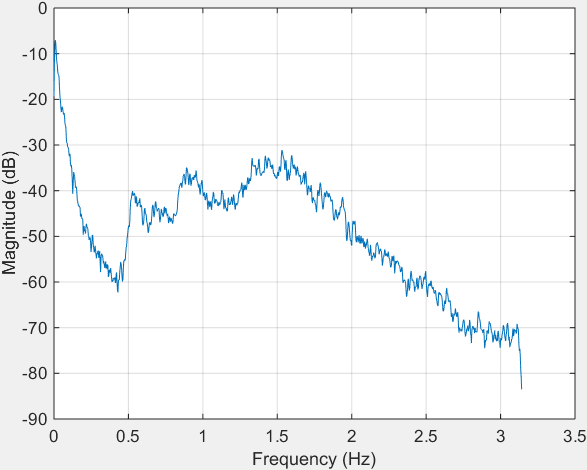
\includegraphics[width=45mm, height=35mm]{image/Ch1/2_noise.png}  \end{minipage}   \\ \hline
 \begin{tabular}[c]{@{}l@{}} Limnodynastes \\ terraereginae  \end{tabular}  &  \begin{minipage}{.3\textwidth} 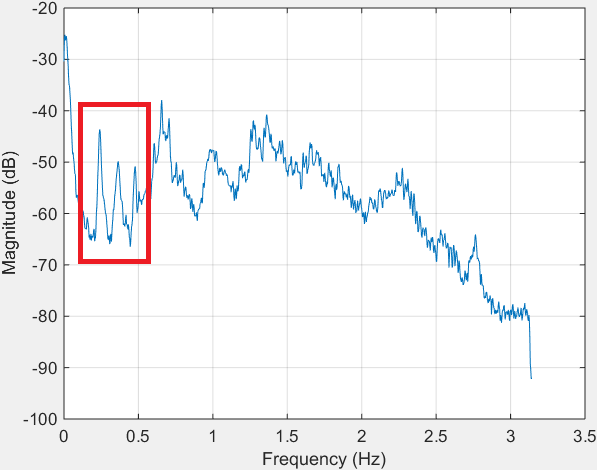
\includegraphics[width=45mm, height=35mm]{image/Ch1/3_signal.png}  \end{minipage}                              &                                             \begin{minipage}{.3\textwidth} 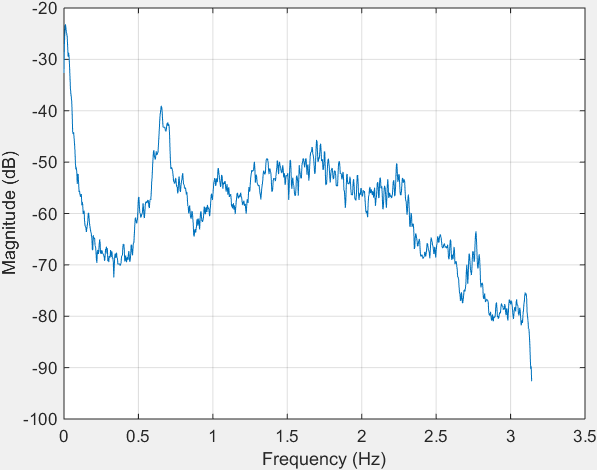
\includegraphics[width=45mm, height=35mm]{image/Ch1/3_noise.png}  \end{minipage}   \\ \hline
Litoria fallax              & \begin{minipage}{.3\textwidth} 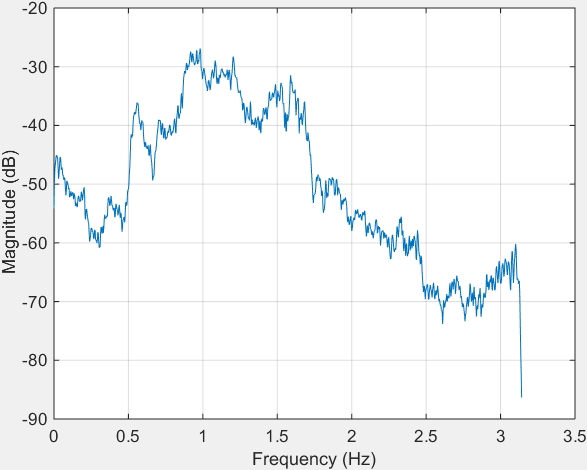
\includegraphics[width=45mm, height=35mm]{image/Ch1/4_signal.png}  \end{minipage}                             &                                               \begin{minipage}{.3\textwidth} 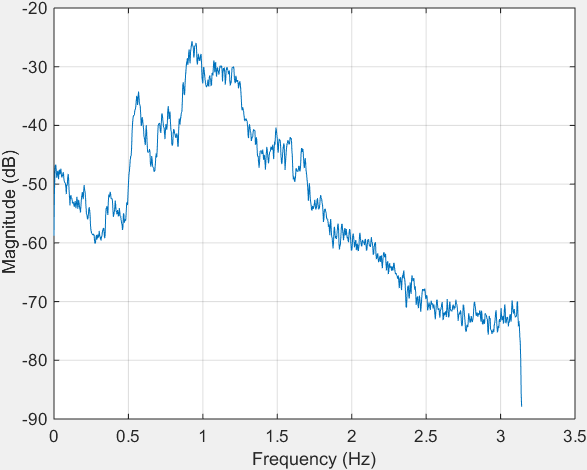
\includegraphics[width=45mm, height=35mm]{image/Ch1/4_noise.png}  \end{minipage} \\ \hline
Litoria nasuta              &   \begin{minipage}{.3\textwidth} 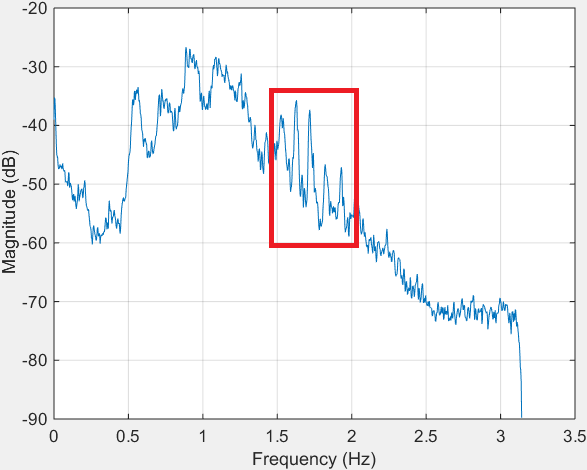
\includegraphics[width=45mm, height=35mm]{image/Ch1/5_signal.png}  \end{minipage}                           &                                               \begin{minipage}{.3\textwidth} 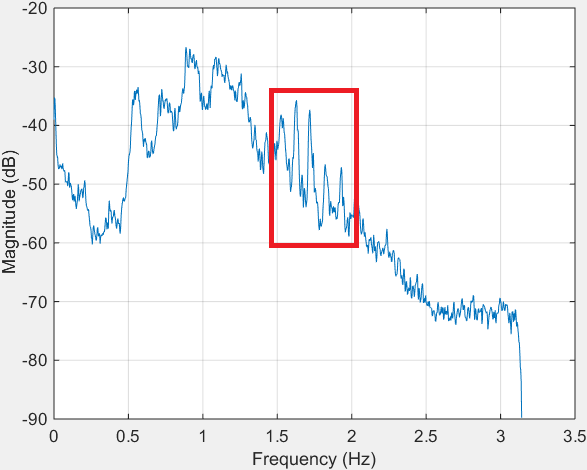
\includegraphics[width=45mm, height=35mm]{image/Ch1/5_signal.png}  \end{minipage} \\ \hline
\end{tabular}
}
\end{table}


\begin{table}[htb!]
\centering
\resizebox{\textwidth}{!}{
\begin{tabular}{lll}
\hline
Litoria rothii              &  \begin{minipage}{.3\textwidth} 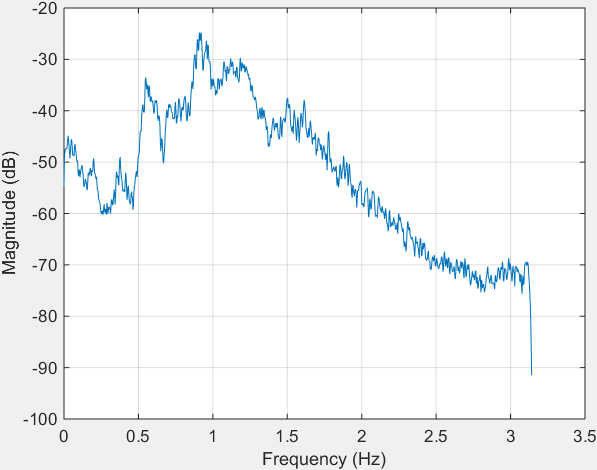
\includegraphics[width=45mm, height=35mm]{image/Ch1/6_signal.png}  \end{minipage}                         &    \begin{minipage}{.3\textwidth} 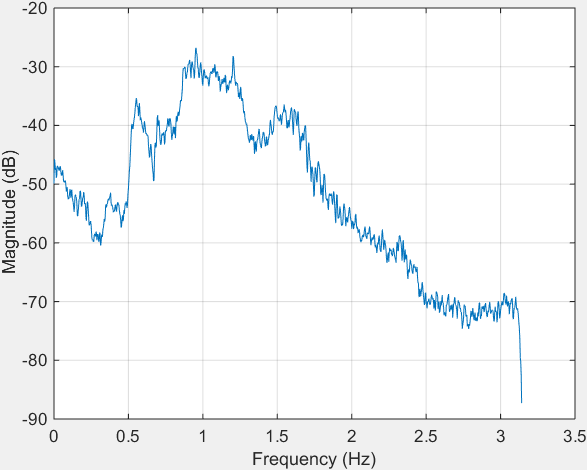
\includegraphics[width=45mm, height=35mm]{image/Ch1/6_noise.png}  \end{minipage}                                           \\ \hline
Litoria rubella             &    \begin{minipage}{.3\textwidth} 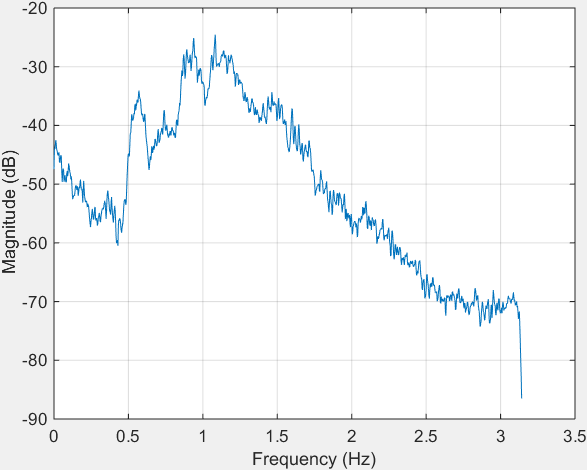
\includegraphics[width=45mm, height=35mm]{image/Ch1/7_signal.png}  \end{minipage}                               &                                               \begin{minipage}{.3\textwidth} 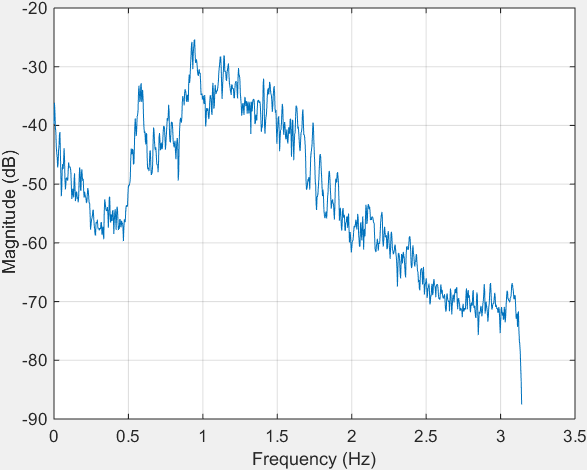
\includegraphics[width=45mm, height=35mm]{image/Ch1/7_noise.png}  \end{minipage} \\ \hline
Uperolela mimula            &   \begin{minipage}{.3\textwidth} 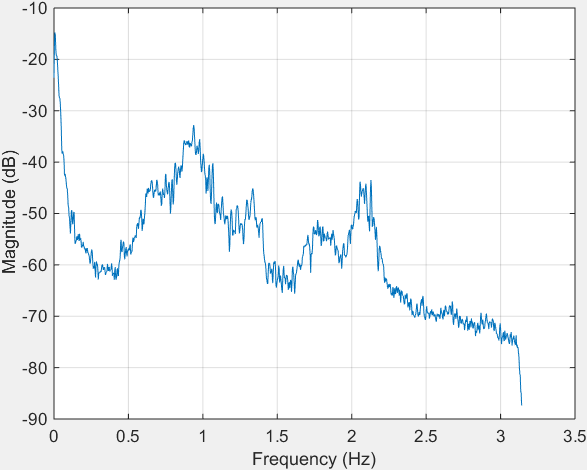
\includegraphics[width=45mm, height=35mm]{image/Ch1/8_signal.png}  \end{minipage}                              &                                             \begin{minipage}{.3\textwidth} 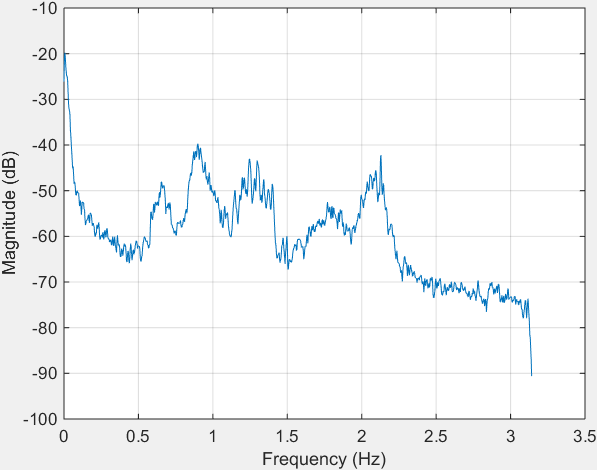
\includegraphics[width=45mm, height=35mm]{image/Ch1/8_noise.png}  \end{minipage} \\ \hline\hline
\end{tabular}
}
\end{table}

\subsection{Frog call classification}

For a frog call classification system, it often consists of four parts (Figure.~\ref{fig:Ch1_flowchart}) : (1) pre-processing, which includes signal processing and noise reduction; (2) syllable segmentation, which is used to generate basic classification unit for frog calls; (3) feature extraction; (4) classification.  



\begin{figure}[htb!]
\centering
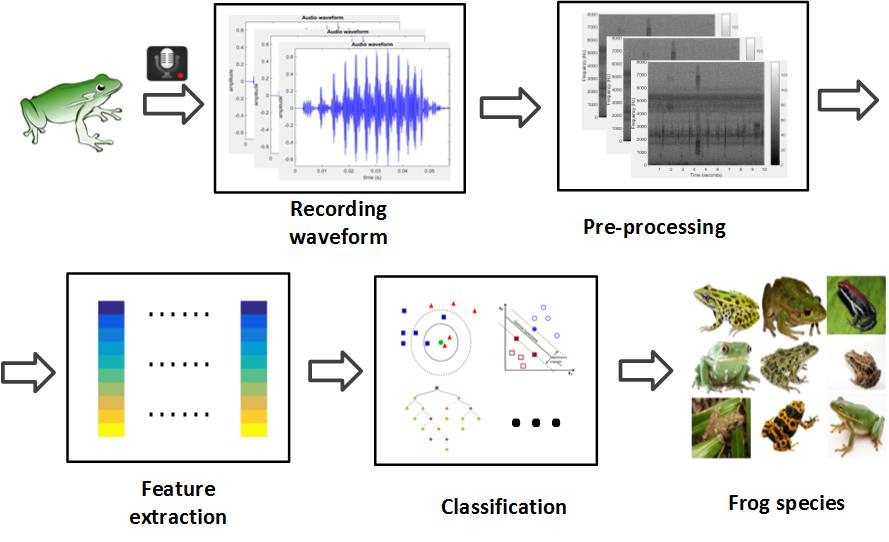
\includegraphics[width=\textwidth]{image/Ch1/flowchart.jpg}
\caption[Flowchart of frog call classification]{Flowchart of frog call classification}
\label{fig:Ch1_flowchart}
\end{figure}


\subsection{Research problem}
Most datasets used in previous frog call classification studies assumes that there is only one frog species exist in each individual recordings. However, these resulting frog calls cannot reflect the characteristics of frog vocalisations in real-world situations, such as background noise, frog chorus. To develop a robust frog call classification system for environmental recordings, two main challenges have been identified. 


\noindent \textbf{Challenge 1}: Most previous work studied frog call classification using high SNR recordings, the first challenge is thus to further improve the classification performance using high SNR recordings. Various acoustic features have been investigated for the classification of frog calls in high SNR recordings. Since our work finally aims to classify frog calls in low SNR recordings, most features that can successfully classify high SNR recordings cannot perform well for low SNR recordings. Consequently, it is still a big challenge to develop robust acoustic features to classify frog species in low SNR recordings. 

\noindent \textbf{Challenge 2}: Another challenge is the classification framework for studying frog vocalisations in low SNR recordings. Since most previous work assumed that each individual recording consists of only one frog species, a single-instance single-label (SISL) framework is suitable for classifying frog calls in those recordings. However, due to the different characters of low SNR recordings, which consist of more than one frog species, the SISL framework is no longer suitable. Therefore, different classification frameworks need to be investigated to study frog vocalisations in low SNR recordings.



\subsection{Research questions}
The research questions are developed in order to solve the aforementioned problems, which can be categorised into three parts. 

 \begin{enumerate}
     \item which acoustic features used for addressing high SNR recordings can be transplanted to study low SNR recordings?
     \item How to develop acoustic features to classify frog calls in low SNR recordings?
     \item How to adopt machine learning techniques to classify simultaneous overlapping frog calls?
  \end{enumerate}




\subsection{Aims and objectives}
This thesis aims to develop a robust frog call classification system to monitor the environment. For high SNR recordings, we want to improve the classification performance. As for the low SNR recordings, we plan to design novel frameworks to classify multiple simultaneously vocalising frog species. With our classification results, ecologists can then make decisions on how to protect and improve the health of frog populations. The specific research objectives are listed below.


\begin{enumerate}

\item	To improve the current representation schemes for modelling frog calls in high SNR recordings

\item 	To develop robust feature extraction methods for low SNR recordings for frog call classification

\item   To investigate machine learning techniques (MIML learning and ML learning) to tackle the frog call classification problem in low SNR recordings

\end{enumerate}
 
 
 
\subsection{Significance and contributions}
For the development of sensor techniques, acoustic sensors have been widely deployed in the field for surveying vocalising animals. Different from recordings collected in the constrained environment, recordings collected in the field often have low SNR and consist of multiple simultaneous vocalising frog species. In this dissertation, we first investigate the high SNR recordings to further improve the classification performance of frog recordings with high SNR. 
Then, those features that can be used for studying frog calls in low SNR recordings are transplanted from high SNR recordings for further analysis.
Since field recordings often consists of multiple simultaneous vocalising frog species, both MIML and ML learning are used for the classification of those low SNR field recordings. Meanwhile, the frog calling activity can also be monitored based on the MIML and ML classification results.
With our developed frog call classification frameworks, ecologists can then analyse frogs by collecting audio data. It will significantly reduce the expert labour cost for monitoring frog calling activity of a particular area. The monitoring result can also help reveal the importance of environment protection, which can be achieved via studying the correlation between the frog calling activity and weather variables. 

 
 
\subsection{Thesis structure} 
 
This thesis consists of eight chapters. Chapter \ref{cha:cha1Introduction} described the background, motivation and contributions of the thesis. Chapter \ref{cha:cha2LiteratureReview} reviews the literature related to frog call classification. Chapter \ref{cha:cha3Method} discusses a number of feature extraction approaches in detail. Also various classification techniques used in this research will be explained, so one can understand the strategy employed for each classifier. Chapter \ref{cha:cha4EnhancedFeature} discusses the implementation of frog call classification by syllable features. Chapter \ref{cha:cha5Wavelet} discusses wavelet analysis for frog call classification. Chapter \ref{cha:cha6MIML} discusses the use of multiple-instance multiple-label framework for frog call classification. Chapter \ref{cha:cha7ML} discusses the multiple-label learning for frog call classification. Chapter \ref{cha:cha8Conclusions} concludes this research and recommends possible directions in future work.

